\documentclass{article}

\usepackage{graphicx}
\usepackage[margin=1in]{geometry}
\usepackage{booktabs}
\usepackage{float}
\usepackage{amsmath}
\usepackage[hidelinks]{hyperref}

\begin{document}

\title{Rotation-Invariant Composite Kernel Findings}
\author{}
\date{21 February 2026}
\maketitle

\section*{Questions}
\begin{enumerate}
    \item \hyperlink{ans1}{How does the 4-right-angle-averaged invariant kernel perform across rotations from $0^\circ$ to $360^\circ$ with a $10^\circ$ step?}
    \item \hyperlink{ans2}{Would the same kernel perform similarly on a newly generated set of train/validation/test patches?}
    \item \hyperlink{ans3}{How does the invariant kernel averaged over rotations every $10^\circ$ look, and how does it perform?}
\end{enumerate}

\section*{Rotation-Invariant Kernel Visualization}
\begin{figure}[H]
    \centering
    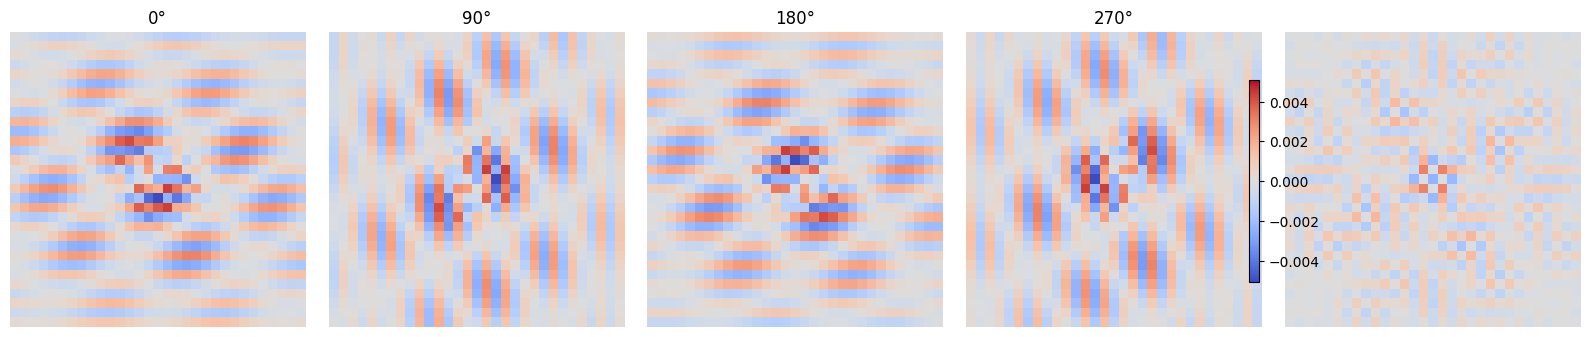
\includegraphics[width=0.85\linewidth]{../results/exp_022_mmr_nperFamily500_nComposition1250/rotation_invariant_kernel.png}
    \caption{Invariant kernel created by averaging right rotation angles.}
\end{figure}

\section*{Data Notes}
\begin{itemize}
    \item The evaluations in this report use \textbf{newly generated patch splits} from the dataset.
    \item The right-angle experiment in Question 2 and the every-$10^\circ$-averaged-kernel experiment in Question 3 use $N=1750$ test samples (patches).
    \item In all cases, evaluation uses the kernel that was generated from the older patch set in order to check it's performance on unseen patches of data.
\end{itemize}

\section*{Results}
\subsection*{\hypertarget{ans1}{1. 4-right-angle-averaged invariant kernel performance from $0^\circ$ to $360^\circ$ (step $10^\circ$)}}
\textbf{Clarification relative to the 18 February 2026 report:}
In the 18 February report, the table and rotation deltas were computed only with respect to the \textbf{invariant} model at test $0^\circ$. In this 21 February report, we keep that comparison and also report deltas with respect to the original \textbf{non-invariant kernel}.

\vspace{0.5em}
This every-$10^\circ$ experiment was evaluated on a \textbf{newly generated patch} of data, while using the kernel that was generated from the \textbf{older patch} set.\footnote{For invariant-kernel results evaluated on the same patch split that was used to generate/train the kernel (including the original composite-kernel baseline), see Table~\ref{tab:same_patch_right_angle} in \hyperref[app:same_patch]{Appendix~\ref*{app:same_patch}}.}

\vspace{0.5em}
\textbf{Summary of every-$10^\circ$ results:}
\begin{itemize}
    \item Evaluated at $0^\circ, 10^\circ, \ldots, 350^\circ$ (with $360^\circ \equiv 0^\circ$).
    \item ACC range: $0.809091$ to $0.826738$; AUC range: $0.884694$ to $0.898277$.
    \item Error difference vs \textbf{invariant} $0^\circ$ baseline: $\Delta E(\theta)\in[-0.017647,\,0.000000]$.
    \item Error difference vs \textbf{original non-invariant} baseline: $\Delta E(\theta)\in[-0.011765,\,+0.005882]$.
    \item Full angle-by-angle values are listed in \hyperref[app:every10_four]{Appendix~\ref*{app:every10_four}}.
\end{itemize}

\begin{figure}[H]
    \centering
    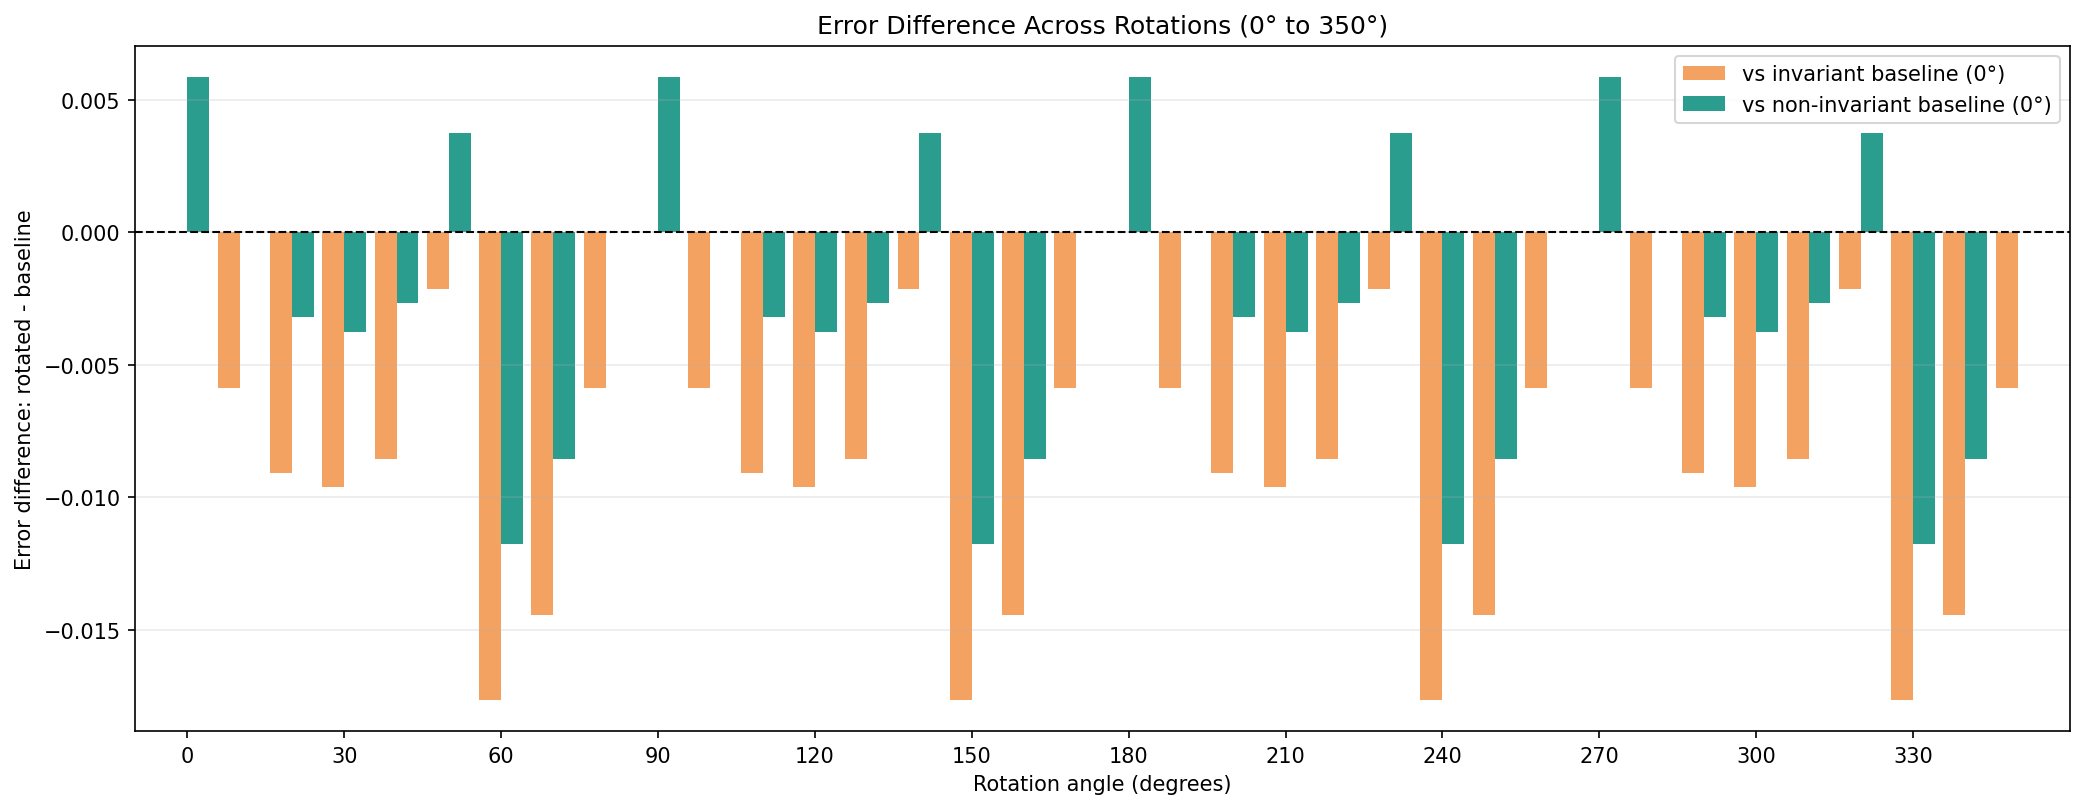
\includegraphics[width=\linewidth]{figures/rotation_error_difference_barplot.png}
    \caption{Bar plot of error difference $\Delta E(\theta)=E(\theta)-E_{\text{baseline}}$ from $0^\circ$ to $350^\circ$. Orange bars compare each rotated invariant-kernel result to the invariant baseline at $0^\circ$; green bars compare to the original non-invariant baseline at $0^\circ$. \textbf{Positive values mean higher error than the baseline.}}
\end{figure}

\subsection*{\hypertarget{ans2}{2. Performance on a newly generated patch split}}

\textbf{Rotation-invariant kernel results:}
\begin{center}
\begin{tabular}{lcc}
\toprule
Evaluation & Test AUC & Test ACC \\
\midrule
Original composite kernel (non-invariant) no-rotation & 0.893287 & 0.814973 \\
Invariant kernel, no-rotation & 0.875518 & 0.800571 \\
Invariant kernel, rotated $90^\circ$ & 0.875518 & 0.800571 \\
Invariant kernel, rotated $180^\circ$ & 0.875518 & 0.800571 \\
Invariant kernel, rotated $270^\circ$ & 0.875518 & 0.800571 \\
\bottomrule
\end{tabular}
\end{center}

\vspace{0.5em}
\textbf{Rotation deltas (rotated $-$ invariant kernel at test $0^\circ$):}
\begin{itemize}
    \item $90^\circ$: $\Delta$AUC $= +0.000000$, $\Delta$ACC $= +0.000000$
    \item $180^\circ$: $\Delta$AUC $= +0.000000$, $\Delta$ACC $= +0.000000$
    \item $270^\circ$: $\Delta$AUC $= +0.000000$, $\Delta$ACC $= +0.000000$
\end{itemize}
This means that the invariant kernel is stable across right-angle rotations.

\vspace{0.5em}
\textbf{Difference vs original non-invariant kernel:}
\[
\Delta \text{AUC} = 0.875518 - 0.893287 = -0.017769,\quad
\Delta \text{ACC} = 0.800571 - 0.814973 = -0.014402
\]
\begin{itemize}
    \item AUC decrease: $0.017769$.
    \item ACC decrease: $0.014402$.
    \item Even with newly generated train/validation/test patches, the kernel trained on an older patch set still performs relatively close to the non-invariant baseline.
\end{itemize}

\subsection*{\hypertarget{ans3}{3. 10$^\circ$-averaged invariant kernel: visualization and performance}}
In this experiment, the invariant kernel is created by averaging rotations at $0^\circ,10^\circ,\ldots,350^\circ$, then evaluated on a newly generated split.

\begin{figure}[H]
    \centering
    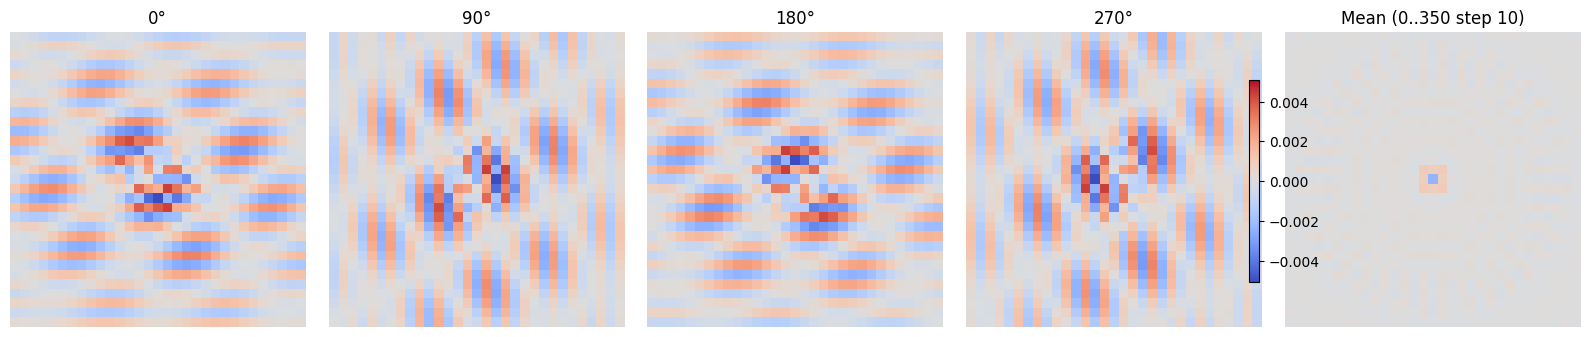
\includegraphics[width=0.85\linewidth]{../results/exp_022_mmr_nperFamily500_nComposition1250/rotation_invariant_kernel_10.png}
    \caption{Invariant kernel created by averaging rotations every $10^\circ$ ($0^\circ$ to $350^\circ$).}
\end{figure}

\begin{figure}[H]
    \centering
    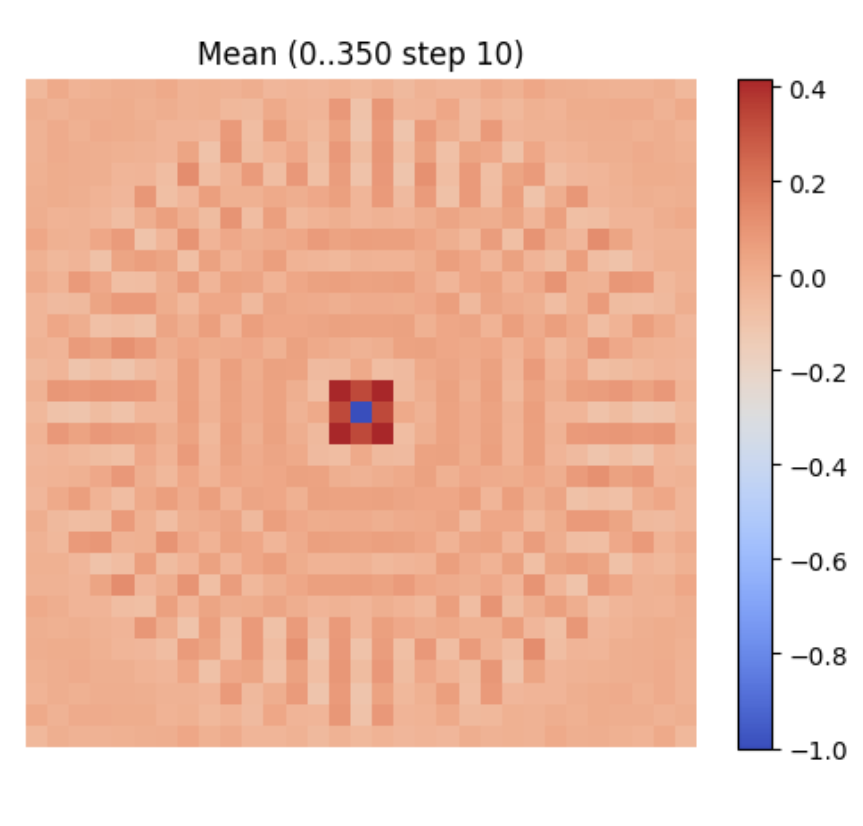
\includegraphics[width=0.32\linewidth]{figures/ivariant_kernle_10_step.png}
    \caption{Additional visualization for the every-$10^\circ$ averaged invariant kernel.}
\end{figure}

\begin{figure}[H]
    \centering
    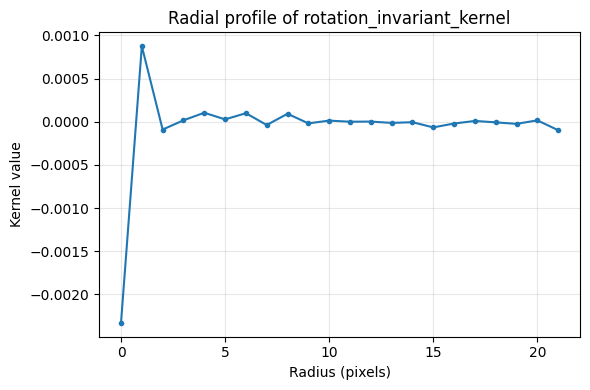
\includegraphics[width=0.52\linewidth]{../results/exp_022_mmr_nperFamily500_nComposition1250/rotation_invariant_kernel_radial_profile.png}
    \caption{Radial profile of the same invariant kernel, showing mean kernel value as a function of radius from the kernel center.}
\end{figure}

\textbf{Performance summary (this run):}
\begin{center}
\begin{tabular}{lcc}
\toprule
Evaluation & Test AUC & Test ACC \\
\midrule
Original composite kernel (non-invariant), no rotation & 0.893287 & 0.814973 \\
10$^\circ$-averaged invariant kernel, test rot $0^\circ$ & 0.871238 & 0.798857 \\
10$^\circ$-averaged invariant kernel, test rot $90^\circ$ & 0.871237 & 0.798857 \\
10$^\circ$-averaged invariant kernel, test rot $180^\circ$ & 0.871237 & 0.798857 \\
10$^\circ$-averaged invariant kernel, test rot $270^\circ$ & 0.871235 & 0.798857 \\
\bottomrule
\end{tabular}
\end{center}

\vspace{0.5em}
\textbf{Summary points:}
\begin{itemize}
    \item Across rotations $0^\circ$ to $350^\circ$, AUC ranges from $0.859495$ to $0.871238$ and ACC ranges from $0.782857$ to $0.801714$.
    \item Deltas vs test-rotation original ($0^\circ$):
    \[
    \Delta \text{AUC}\in[-0.011743,\,0.000000],\quad
    \Delta \text{ACC}\in[-0.016000,\,+0.002857]
    \]
    \item Compared with the 4-right-angle-averaged kernel in Question 2 at $0^\circ$ (AUC $=0.875518$, ACC $=0.800571$), this 10$^\circ$-averaged kernel performs worse (AUC lower by $0.004280$, ACC lower by $0.001714$).
    \item Full angle-by-angle values for this 10$^\circ$-averaged kernel are provided in \hyperref[app:every10_tenavg]{Appendix~\ref*{app:every10_tenavg}}.
\end{itemize}

\section*{Findings}
\begin{itemize}
    \item For right-angle rotations, the invariant kernel is stable: $0^\circ$, $90^\circ$, $180^\circ$, and $270^\circ$ give identical AUC/ACC in the new-split run.
    \item Compared with the non-invariant composite baseline, the invariant result on the new split is slightly lower (AUC by about $1.99\%$ relative and ACC by about $1.77\%$ relative).
    \item In the every-$10^\circ$ experiment, angle-wise behavior and error-difference trends are summarized in Question 1 and detailed in \hyperref[app:every10_four]{Appendix~\ref*{app:every10_four}}.
    \item The 10$^\circ$-averaged invariant kernel is also stable at right angles, but it performs worse than the 4-right-angle-averaged kernel.
    \item Overall, transferring the kernel to a newly generated patch split still yields relatively close performance.
\end{itemize}

\section*{Conclusion}
The invariant kernel remains rotation-stable at right-angle rotations on a newly generated split, and it stays relatively close to the non-invariant composite baseline despite being transferred from an older patch set. The every-$10^\circ$ sweep shows consistent angle-wise behavior. The kernel averaged over every $10^\circ$ performs worse than the 4-right-angle-averaged kernel in this run. Full values are reported in \hyperref[app:every10_four]{Appendix~\ref*{app:every10_four}} and \hyperref[app:every10_tenavg]{Appendix~\ref*{app:every10_tenavg}}.

\newpage

\appendix
\section{Same-Patch Right-Angle Evaluation}\label{app:same_patch}
\textbf{Setup note.} The table below reports the right-angle evaluation on the same patch split used when the kernel was generated (comparable to the 18 February).

\begin{table}[H]
    \centering
    \begin{tabular}{lcc}
    \toprule
    Evaluation & Test AUC & Test ACC \\
    \midrule
    Original composite kernel (non-invariant) & 0.893287 & 0.814973 \\
    Invariant kernel, test rotated $0^\circ$ & 0.890774 & 0.809091 \\
    Invariant kernel, test rotated $90^\circ$ & 0.890774 & 0.809091 \\
    Invariant kernel, test rotated $180^\circ$ & 0.890774 & 0.809091 \\
    Invariant kernel, test rotated $270^\circ$ & 0.890773 & 0.809091 \\
    \bottomrule
    \end{tabular}
    \caption{Invariant-kernel right-angle results on the same patch split used for kernel generation/training.}
    \label{tab:same_patch_right_angle}
\end{table}

\section{\texorpdfstring{Every-$10^\circ$ Evaluation}{Every-10-degree Evaluation}}\label{app:every10_four}
\textbf{Setup note.} The rotation-invariant kernel was created by averaging the composite kernel at $0^\circ$, $90^\circ$, $180^\circ$, and $270^\circ$. The every-$10^\circ$ evaluation below was run on a newly generated patch split, while using the kernel generated from the older patch set.

\textbf{Detailed outputs:} The complete angle-by-angle results corresponding to the main-results bar plot are listed below.

\textbf{Notation note:} In the raw block below, \texttt{dAUC} and \texttt{dACC} are extra right-side columns computed against the invariant-kernel average over $0^\circ$, $90^\circ$, $180^\circ$, and $270^\circ$.

\begin{verbatim}
Rotation-invariant kernel results (every 10 deg) with delta columns:
  baseline(avg 0/90/180/270) | AUC=0.890774 ACC=0.809091
  rot   0 | AUC=0.890774 ACC=0.809091 | dAUC=+0.000000 dACC=+0.000000
  rot  10 | AUC=0.884694 ACC=0.814973 | dAUC=-0.006080 dACC=+0.005882
  rot  20 | AUC=0.885241 ACC=0.818182 | dAUC=-0.005533 dACC=+0.009091
  rot  30 | AUC=0.892792 ACC=0.818717 | dAUC=+0.002018 dACC=+0.009626
  rot  40 | AUC=0.896533 ACC=0.817647 | dAUC=+0.005759 dACC=+0.008556
  rot  50 | AUC=0.893674 ACC=0.811230 | dAUC=+0.002900 dACC=+0.002139
  rot  60 | AUC=0.897000 ACC=0.826738 | dAUC=+0.006226 dACC=+0.017647
  rot  70 | AUC=0.898276 ACC=0.823529 | dAUC=+0.007502 dACC=+0.014438
  rot  80 | AUC=0.892234 ACC=0.814973 | dAUC=+0.001460 dACC=+0.005882
  rot  90 | AUC=0.890774 ACC=0.809091 | dAUC=+0.000000 dACC=+0.000000
  rot 100 | AUC=0.884694 ACC=0.814973 | dAUC=-0.006080 dACC=+0.005882
  rot 110 | AUC=0.885241 ACC=0.818182 | dAUC=-0.005533 dACC=+0.009091
  rot 120 | AUC=0.892791 ACC=0.818717 | dAUC=+0.002017 dACC=+0.009626
  rot 130 | AUC=0.896534 ACC=0.817647 | dAUC=+0.005760 dACC=+0.008556
  rot 140 | AUC=0.893675 ACC=0.811230 | dAUC=+0.002901 dACC=+0.002139
  rot 150 | AUC=0.897000 ACC=0.826738 | dAUC=+0.006226 dACC=+0.017647
  rot 160 | AUC=0.898277 ACC=0.823529 | dAUC=+0.007503 dACC=+0.014438
  rot 170 | AUC=0.892234 ACC=0.814973 | dAUC=+0.001460 dACC=+0.005882
  rot 180 | AUC=0.890774 ACC=0.809091 | dAUC=+0.000000 dACC=+0.000000
  rot 190 | AUC=0.884694 ACC=0.814973 | dAUC=-0.006080 dACC=+0.005882
  rot 200 | AUC=0.885241 ACC=0.818182 | dAUC=-0.005533 dACC=+0.009091
  rot 210 | AUC=0.892792 ACC=0.818717 | dAUC=+0.002018 dACC=+0.009626
  rot 220 | AUC=0.896533 ACC=0.817647 | dAUC=+0.005759 dACC=+0.008556
  rot 230 | AUC=0.893673 ACC=0.811230 | dAUC=+0.002899 dACC=+0.002139
  rot 240 | AUC=0.897000 ACC=0.826738 | dAUC=+0.006226 dACC=+0.017647
  rot 250 | AUC=0.898277 ACC=0.823529 | dAUC=+0.007503 dACC=+0.014438
  rot 260 | AUC=0.892234 ACC=0.814973 | dAUC=+0.001460 dACC=+0.005882
  rot 270 | AUC=0.890773 ACC=0.809091 | dAUC=-0.000001 dACC=+0.000000
  rot 280 | AUC=0.884694 ACC=0.814973 | dAUC=-0.006080 dACC=+0.005882
  rot 290 | AUC=0.885241 ACC=0.818182 | dAUC=-0.005533 dACC=+0.009091
  rot 300 | AUC=0.892792 ACC=0.818717 | dAUC=+0.002018 dACC=+0.009626
  rot 310 | AUC=0.896533 ACC=0.817647 | dAUC=+0.005759 dACC=+0.008556
  rot 320 | AUC=0.893673 ACC=0.811230 | dAUC=+0.002899 dACC=+0.002139
  rot 330 | AUC=0.897000 ACC=0.826738 | dAUC=+0.006226 dACC=+0.017647
  rot 340 | AUC=0.898276 ACC=0.823529 | dAUC=+0.007502 dACC=+0.014438
  rot 350 | AUC=0.892234 ACC=0.814973 | dAUC=+0.001460 dACC=+0.005882
\end{verbatim}

\section{\texorpdfstring{Every-$10^\circ$-Averaged Kernel Evaluation}{Every-10-degree-Averaged Kernel Evaluation}}\label{app:every10_tenavg}
\textbf{Setup note.} In this experiment, the invariant kernel is created by averaging rotated versions of the kernel at every $10^\circ$ from $0^\circ$ to $350^\circ$, and then evaluating on the newly generated patch split.
\textbf{Notation note.} In the block below, \texttt{dAUC} and \texttt{dACC} are \texttt{Deltas vs original} (rotation $0^\circ$), shown as right-side columns.

\begin{verbatim}
Saved composite test metrics from results.json:
  AUC=0.893287 ACC=0.814973

Rotation-invariant kernel results (every 10°) with delta columns:
  baseline(original rot 0) | AUC=0.871238 ACC=0.798857
  rot   0 | AUC=0.871238 ACC=0.798857 | dAUC=+0.000000 dACC=+0.000000
  rot  10 | AUC=0.862297 ACC=0.787429 | dAUC=-0.008941 dACC=-0.011429
  rot  20 | AUC=0.859495 ACC=0.782857 | dAUC=-0.011743 dACC=-0.016000
  rot  30 | AUC=0.868592 ACC=0.796571 | dAUC=-0.002646 dACC=-0.002286
  rot  40 | AUC=0.867827 ACC=0.801714 | dAUC=-0.003411 dACC=+0.002857
  rot  50 | AUC=0.867346 ACC=0.793714 | dAUC=-0.003892 dACC=-0.005143
  rot  60 | AUC=0.870454 ACC=0.800571 | dAUC=-0.000785 dACC=+0.001714
  rot  70 | AUC=0.863602 ACC=0.789143 | dAUC=-0.007636 dACC=-0.009714
  rot  80 | AUC=0.860216 ACC=0.789143 | dAUC=-0.011022 dACC=-0.009714
  rot  90 | AUC=0.871237 ACC=0.798857 | dAUC=-0.000001 dACC=+0.000000
  rot 100 | AUC=0.862297 ACC=0.787429 | dAUC=-0.008941 dACC=-0.011429
  rot 110 | AUC=0.859495 ACC=0.782857 | dAUC=-0.011743 dACC=-0.016000
  rot 120 | AUC=0.868590 ACC=0.796571 | dAUC=-0.002648 dACC=-0.002286
  rot 130 | AUC=0.867827 ACC=0.801714 | dAUC=-0.003411 dACC=+0.002857
  rot 140 | AUC=0.867346 ACC=0.793714 | dAUC=-0.003892 dACC=-0.005143
  rot 150 | AUC=0.870451 ACC=0.800571 | dAUC=-0.000787 dACC=+0.001714
  rot 160 | AUC=0.863606 ACC=0.789143 | dAUC=-0.007633 dACC=-0.009714
  rot 170 | AUC=0.860215 ACC=0.789143 | dAUC=-0.011023 dACC=-0.009714
  rot 180 | AUC=0.871237 ACC=0.798857 | dAUC=-0.000001 dACC=+0.000000
  rot 190 | AUC=0.862297 ACC=0.787429 | dAUC=-0.008941 dACC=-0.011429
  rot 200 | AUC=0.859495 ACC=0.782857 | dAUC=-0.011743 dACC=-0.016000
  rot 210 | AUC=0.868590 ACC=0.796571 | dAUC=-0.002648 dACC=-0.002286
  rot 220 | AUC=0.867827 ACC=0.801714 | dAUC=-0.003411 dACC=+0.002857
  rot 230 | AUC=0.867347 ACC=0.793714 | dAUC=-0.003891 dACC=-0.005143
  rot 240 | AUC=0.870452 ACC=0.800571 | dAUC=-0.000786 dACC=+0.001714
  rot 250 | AUC=0.863602 ACC=0.789143 | dAUC=-0.007636 dACC=-0.009714
  rot 260 | AUC=0.860216 ACC=0.789143 | dAUC=-0.011022 dACC=-0.009714
  rot 270 | AUC=0.871235 ACC=0.798857 | dAUC=-0.000003 dACC=+0.000000
  rot 280 | AUC=0.862297 ACC=0.787429 | dAUC=-0.008941 dACC=-0.011429
  rot 290 | AUC=0.859495 ACC=0.782857 | dAUC=-0.011743 dACC=-0.016000
  rot 300 | AUC=0.868590 ACC=0.796571 | dAUC=-0.002648 dACC=-0.002286
  rot 310 | AUC=0.867827 ACC=0.801714 | dAUC=-0.003411 dACC=+0.002857
  rot 320 | AUC=0.867346 ACC=0.793714 | dAUC=-0.003892 dACC=-0.005143
  rot 330 | AUC=0.870452 ACC=0.800571 | dAUC=-0.000787 dACC=+0.001714
  rot 340 | AUC=0.863602 ACC=0.789143 | dAUC=-0.007636 dACC=-0.009714
  rot 350 | AUC=0.860216 ACC=0.789143 | dAUC=-0.011022 dACC=-0.009714
\end{verbatim}

\end{document}
